\documentclass{article}
\usepackage{ctex} % 添加中文支持包
\usepackage{geometry}
\geometry{margin=2.5cm}
\usepackage{graphicx}
\usepackage{mhchem}
\usepackage{amsmath}
\usepackage{booktabs}
\usepackage{hyperref}
\usepackage{graphicx}
\usepackage{float}
\usepackage{subcaption}
\usepackage{xcolor}

\title{Ex13}

\begin{document}
\newpage

\section{simulink模型修改}
\subsection{替换非线性元件Arrester}

\indent simulink中使用NonLinear Resistor元件实现Arrester会导致simulink求解难以收敛，该问题目前尚未解决。
因此采用替代方案：根据Arrester的I-U特性，使用diode实现Arrester。

\begin{figure}[H] % 使用[H]选项将图片固定在当前位置
 \centering
    \begin{minipage}{0.8\textwidth}
        \centering
         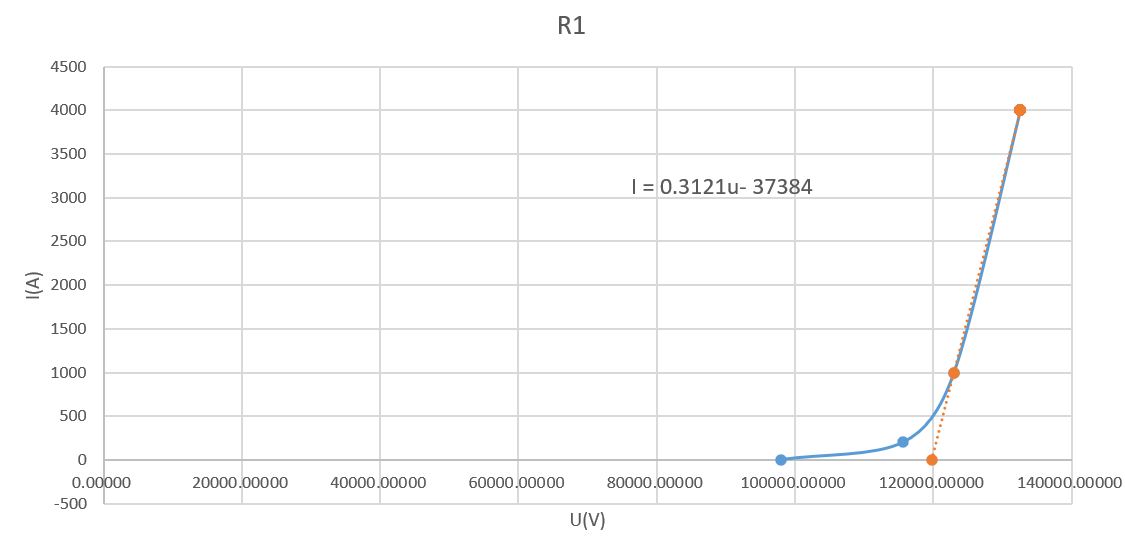
\includegraphics[width=\textwidth, height=0.5\textwidth, keepaspectratio]{R_replace.png}
        
        \label{fig:rotor}
    \end{minipage}
    \hfill
    \begin{minipage}{0.8\textwidth}
        \centering
        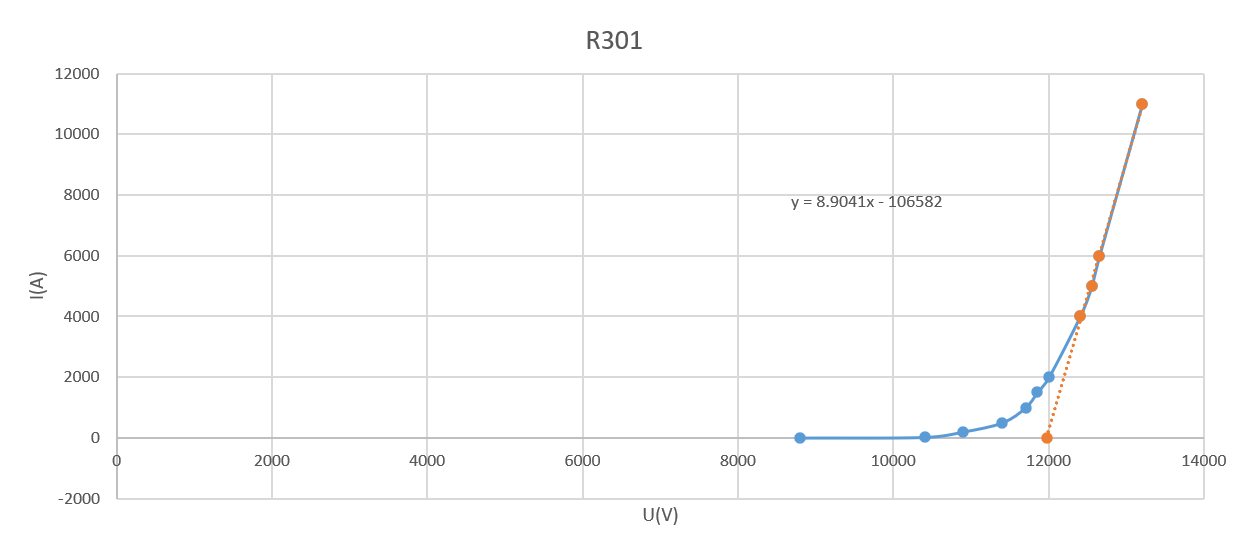
\includegraphics[width=\textwidth, height=0.5\textwidth, keepaspectratio]{R301_replace.png}
        
        \label{fig:stator}
    \end{minipage}
    
    \caption{I-U特性}
    \label{fig:motor_structures}
\end{figure}

\subsection{Arrester、Bridge反接}
\indent 需将原simulink模型中所有Arrester元件和Bridge反接。

\subsection{参数修改}
\indent 原simulink模型中所有Arrester元件电压基值有误。\newline
\indent 原simulink模型中所有Bridge - segment - R201/R202/R203/R204/R205/R206: 88 Ohms 修改为 88000 Ohms。\newline
\indent 原simulink模型中所有Bridge - segment - Gto1/Gto2/Gto3/Gto4/Gto5/Gto6 - Ron: 0.226e-6 Ohms 修改为 0.226e-3 Ohms。\newline
\indent 原simulink模型中DC Voltage: 5700 V 修改为 57000 V。

\subsection{Three-Phase Voltage Source修改}
\indent 改用Three-Phase Programmable Voltage Source，在t从0到0.05秒内，电压幅值线性地从0升到设定值。

\begin{figure}[H] % 使用[H]选项将图片固定在当前位置
    \centering
    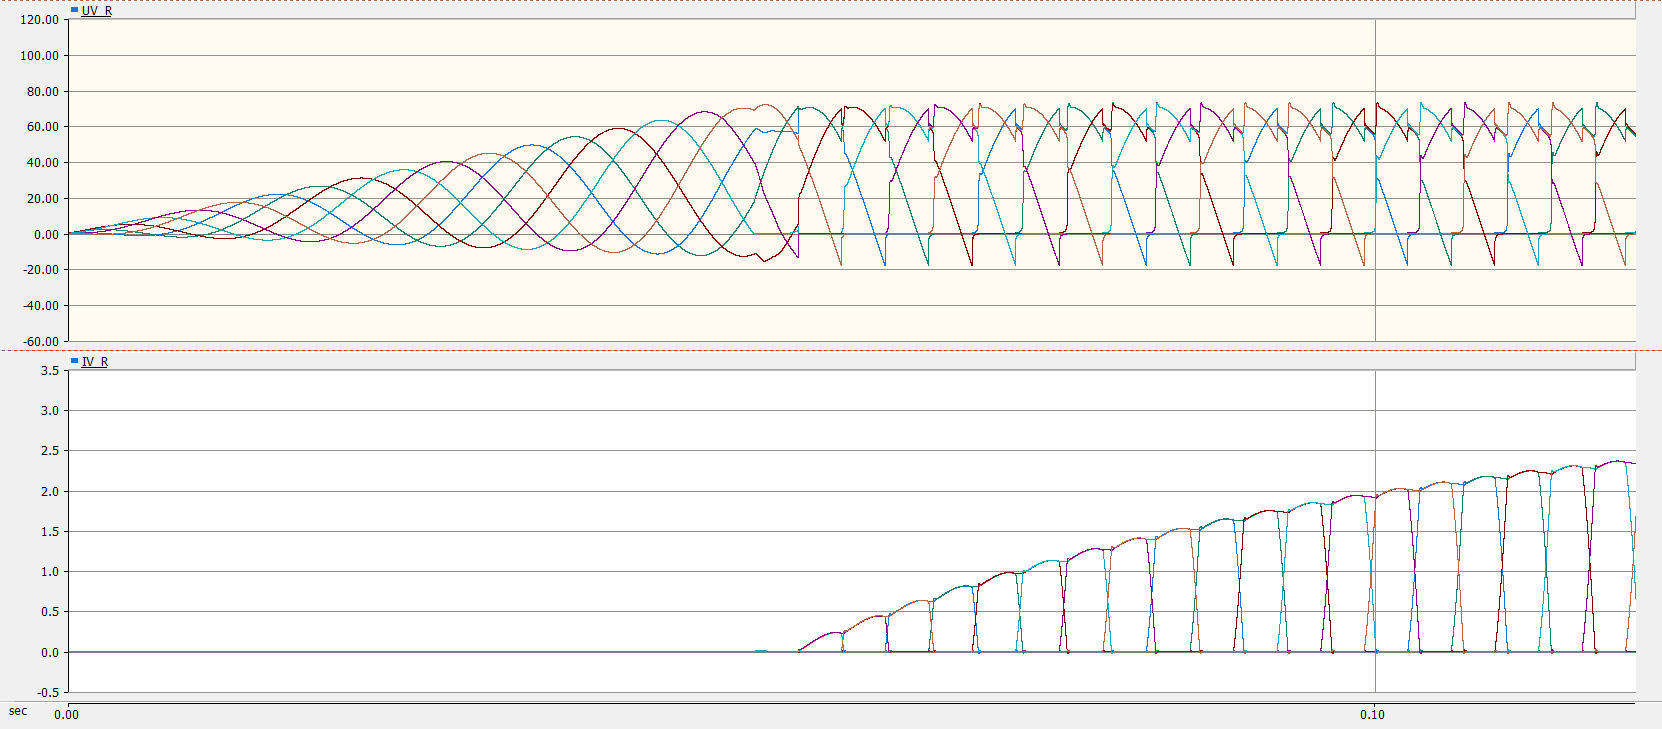
\includegraphics[width=0.8\textwidth]{PSCAD_result.png}
    \caption{PSCAD仿真结果}
    \label{fig:motor_structures}
\end{figure}

\begin{figure}[H] % 使用[H]选项将图片固定在当前位置
 \centering
    \begin{minipage}{0.79\textwidth}
        \centering
         \includegraphics[width=1.0\textwidth,height=0.4\textwidth, keepaspectratio=false]{Simulink_result2.png}
        
        \label{fig:rotor}
    \end{minipage}
    \hfill
    \begin{minipage}{0.79\textwidth}
        \centering
        \includegraphics[width=1.0\textwidth,height=0.4\textwidth, keepaspectratio=false]{Simulink_result1.png}
        
        \label{fig:stator}
    \end{minipage}
    
    \caption{Simulink仿真结果}
    \label{fig:motor_structures}
\end{figure}

\begin{figure}[H] % 使用[H]选项将图片固定在当前位置
    \centering
    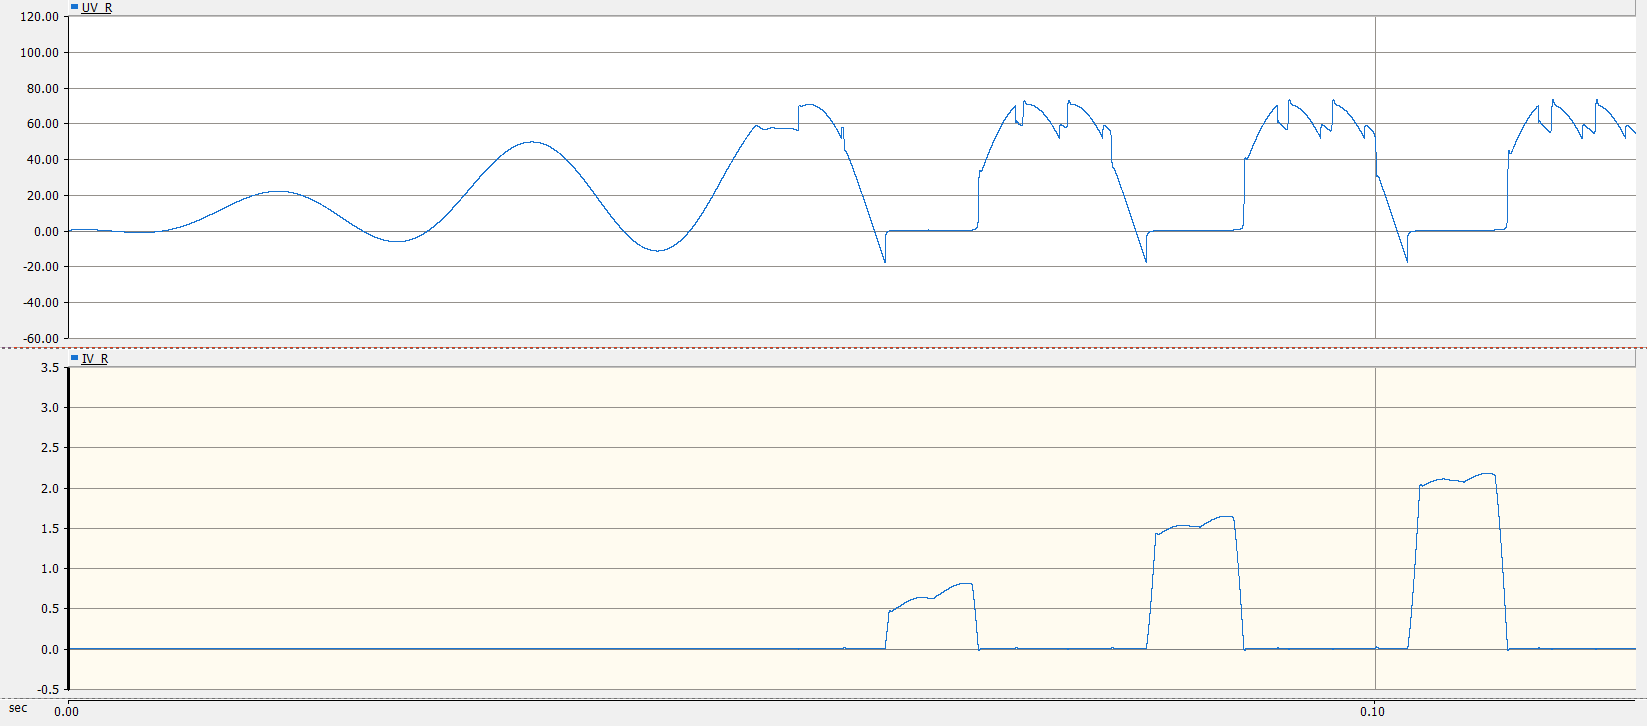
\includegraphics[width=0.8\textwidth]{PSCAD_result_single.png}
    \caption{PSCAD仿真结果}
    \label{fig:motor_structures}
\end{figure}

\begin{figure}[H] % 使用[H]选项将图片固定在当前位置
 \centering
    \begin{minipage}{0.8\textwidth}
        \centering
         \includegraphics[width=1.0\textwidth,height=0.4\textwidth, keepaspectratio=false]{Simulink_result2_single.png}
        
        \label{fig:rotor}
    \end{minipage}
    \hfill
    \begin{minipage}{0.8\textwidth}
        \centering
        \includegraphics[width=1.0\textwidth,height=0.4\textwidth, keepaspectratio=false]{Simulink_result1_single.png}
        
        \label{fig:stator}
    \end{minipage}
    
    \caption{Simulink仿真结果}
    \label{fig:motor_structures}
\end{figure}

\newpage
\section{控制信号}

将PSCAD中的控制信号复制到txt文件中，再由matlab读取。

\section{转换矩阵Req}

\indent Gto、Diode导通时：\indent $u = R \times i + V_{f}$\newline
\indent Gto、Diode截止时：\indent $i = 0$\newline


\section{MOSFET和Diode导通状态判断}

\indent 若控制信号为0，则对应的Gto一定截止。将其余Diode和Dto元件假设导通。\newline
\indent 根据假设的导通情况暂时更新$R_{eq}^{on}, D_{nl}^{on}, C^{on}, D_{l}^{on}, V_{eq}^{on}$， \newline
\indent 求解u，根据每个u和对应元件的Vf以及导通信号判断是否导通。\newline

\section{仿真结果}
\begin{figure}[H] % 使用[H]选项将图片固定在当前位置
    \centering
    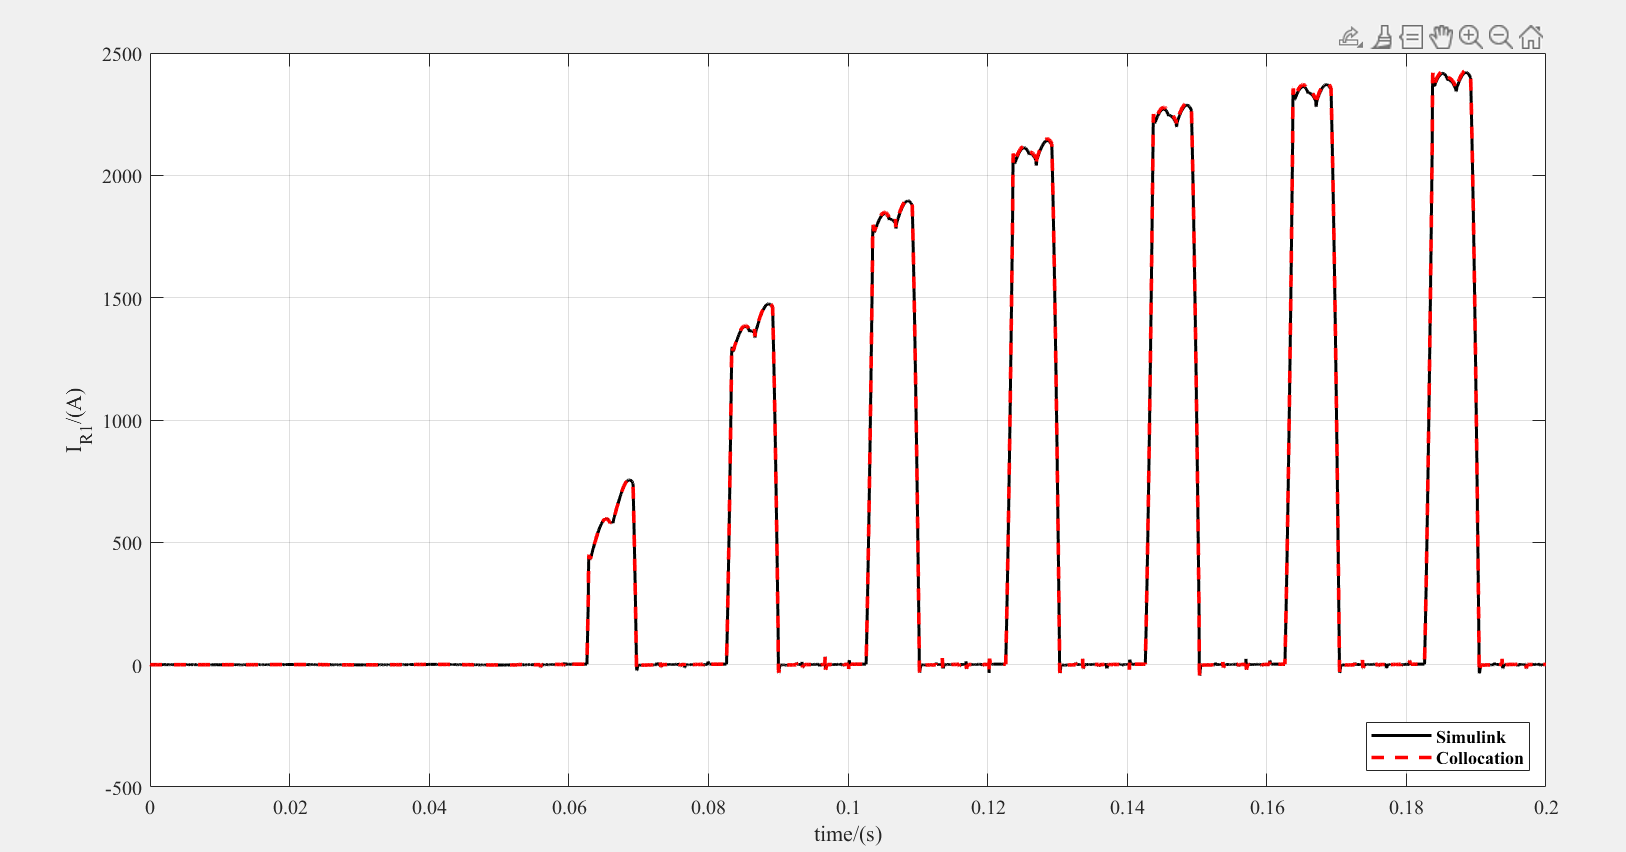
\includegraphics[width=0.8\textwidth]{collocation_res_1.png}
    \caption{I\_R1-时间曲线}
    \label{fig:motor_structures}
\end{figure}

\begin{figure}[H] % 使用[H]选项将图片固定在当前位置
    \centering
    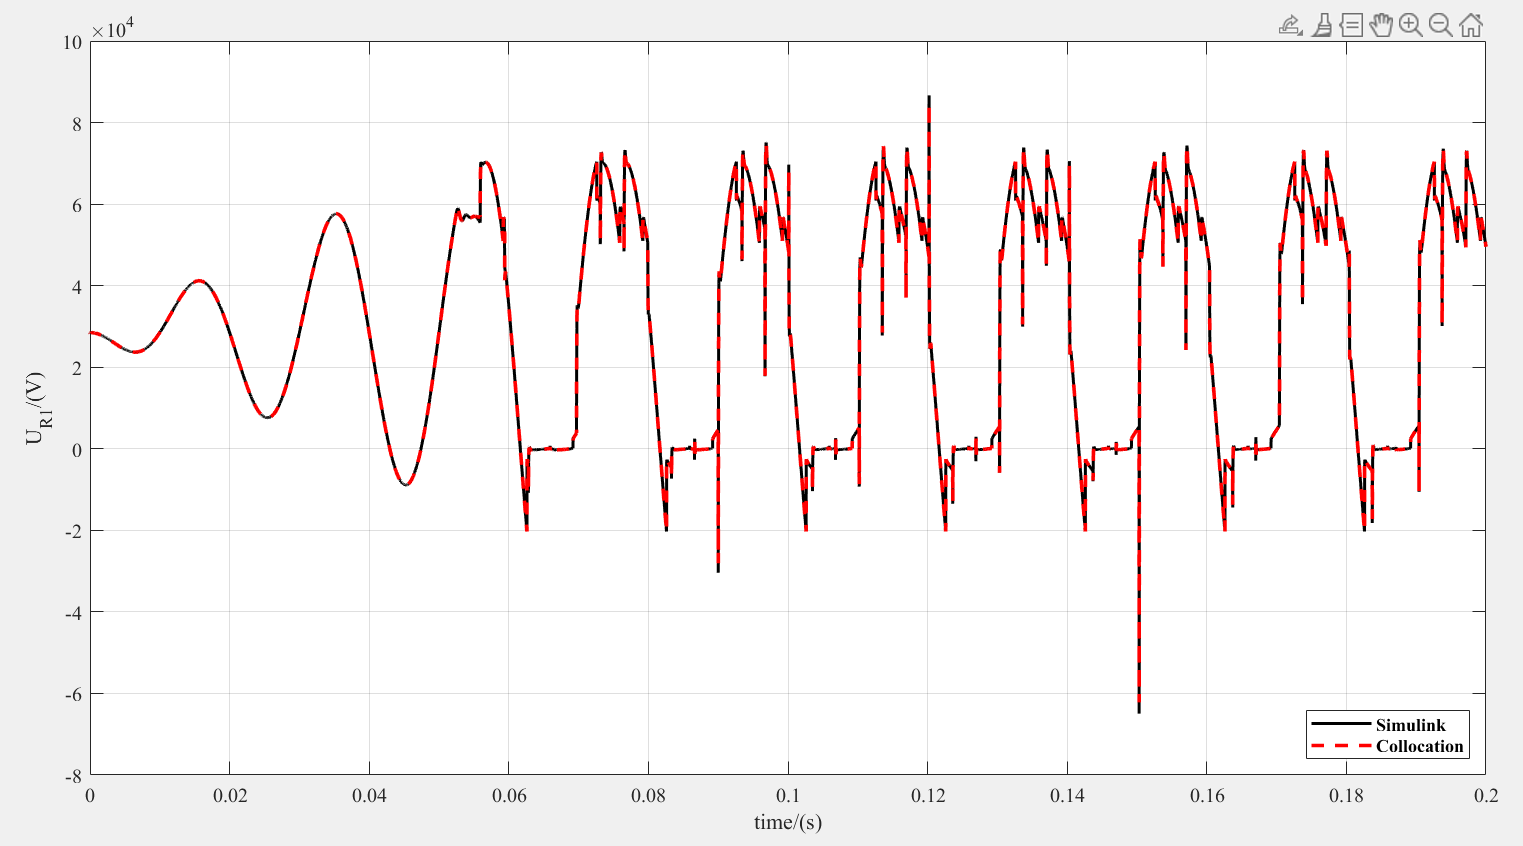
\includegraphics[width=0.8\textwidth]{collocation_res_2.png}
    \caption{U\_R1-时间曲线}
    \label{fig:motor_structures}
\end{figure}

\end{document}
